
\noindent\textbf{5.1. (CLRS 23.1-4)} Dê um exemplo simples de um grafo tal que o conjunto de arestas \{$(u, v)$ : existe um corte $(S, V - S)$ tal que $(u, v)$ é uma aresta de custo mínimo atravessando o corte\} não forma uma MST.\\[6pt]
\textbf{Resposta:} Basta pensarmos em um triângulo com 3 vértices conectados por arestas de mesmo peso $w(e_1) = w(e_2) = w(e_3)$. Independente do corte, nós sempre teremos uma aresta de custo mínimo que não estará na MST pois, do contrário, teríamos um ciclo.

\begin{center}
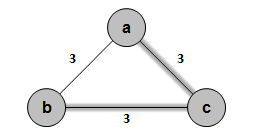
\includegraphics[width=0.35\textwidth]{q8-05-1.png}
\captionof{figure}{Exemplo de grafo onde uma aresta de custo mínimo  não pertence à MST.}
\label{fig:8.5-1-1}
\end{center}